\section{Análise Semântica (\texttt{checker})} \label{section-checker}
O processo de validação semântica no compilador é crucial para garantir a corretude das equações, a consistência de tipos em operações e a resolução adequada de símbolos. Ele é estruturado em dois mecanismos principais: validação de definições de funções e validação de declarações. Esses mecanismos trabalham de forma integrada para garantir que a estrutura do programa esteja em conformidade com as regras semânticas da \texttt{EquationLang}.

Nesta seção, apresentamos essas regras e discutimos como são validadas expressões envolvendo vetores, redefinições de equações e possíveis erros nas definições de BRDFs que inviabilizem a geração de código. A conclusão bem-sucedida dessa etapa de inferência e validação indica que o programa está apto a prosseguir para a fase de geração de código GLSL, conduzida pelo pacote \texttt{emitter}.


\subsection{Funções do Pacote \texttt{checker}}

O pacote \texttt{checker} é responsável por realizar diversas tarefas fundamentais para a validação semântica do compilador. Essas tarefas são descritas detalhadamente a seguir:

\begin{enumerate}
    \item \textbf{Inferência e Anotação de Tipos}:
    Cada expressão na AST possui um campo \verb"ty_inferred" que deve ser preenchido durante essa etapa. Para determinar esses tipos, é necessário realizar a inferência de tipos. Essa tarefa é detalhada na \autoref{subsection-type-inference}. Os tipos possíveis incluem números (\verb"float"), vetores (\verb"vector") e funções.
        O tipo de uma função é representada por um domínio (tipos dos argumentos de entrada) e um contradomínio (tipo do valor de retorno). Exemplos incluem:
        \begin{itemize}
            \item Uma função $f(a, b) = a \cdot b \cdot \vec{1,1,1}$, que recebe dois valores reais e retorna um vetor tridimensional, possui a assinatura:
            \[
            f : \mathbb{R} \times \mathbb{R} \to \mathbb{R}^3.
            \]
            \item O produto vetorial, que combina dois vetores tridimensionais, possui a assinatura:
            \[
            \times : \mathbb{R}^3 \times \mathbb{R}^3 \to \mathbb{R}^3.
            \]
        \end{itemize}
        Essas assinaturas são coletadas durante o processo de inferência para garantir a consistência em expressões de chamada de funções.

    \item \textbf{Compatibilidade de Tipos}:
    O \texttt{checker} também verifica a compatibilidade entre tipos em diferentes contextos do programa. Essa validação assegura que:
    \begin{itemize}
        \item Não sejam realizadas operações indefinidas em \texttt{EquationLang}, como a divisão entre dois vetores.
        \item Não sejam aplicados operadores em tipos incompatíveis, como elevar um número a um vetor ($2^{\vec{n}}$).
        \item Os argumentos de uma função devem pertencer ao domínio esperado pela função. Por exemplo, se a função $\texttt{normalize}(\vec{u})$ retorna um vetor tridimensional ($\mathbb{R}^3$), utilizá-lo como argumento para a função seno, que espera um número escalar ($\mathbb{R}$), seria inválido. Assim, $\sin(\texttt{normalize}(\vec{u}))$ não é permitido.
        \item O tipo do valor de retorno de uma função deve ser compatível com o contexto em que é utilizado.
    \end{itemize}

    \item \textbf{Validação de Definições de Símbolos}:
        Outro papel fundamental do \texttt{checker} é garantir que todos os identificadores, abstraídos em símbolos na \autoref{subsection-symbols-scopes}, utilizados no programa, estejam devidamente definidos antes de serem usados. Essa etapa inclui:
    \begin{itemize}
        \item Identificar declarações ausentes.
        \item Identificar dependência circular.
        \item Certificar-se de que funções obrigatórias, como a BRDF $f$, estejam presentes.
    \end{itemize}
\end{enumerate}

Essas validações são realizadas utilizando as funções do pacote \textit{walker}, e os erros encontrados são reportados usando as funções de erro introduzidas na \autoref{section-lexer}.

% \subsection{Uso do Padrão Visitor}
% @@@ Prefisamos manter essa subseção se já vamos detalhar mais pra frente?@@
%
% Para realizar a validação semântica, o pacote \texttt{walker} é reutilizado, permitindo a travessia modular da AST. Essa abordagem facilita a aplicação recursiva de inferência de tipos, provida pelo, mesmo em expressões aninhadas.
%
% Validações ocorrem nessa traversia e basedo no tipo do nó, a inferencia é feita, discutido na \autoref{subsection-inferencia-tipos} uma operação binária de multiplicação:
% \begin{itemize}
%     \item Se ambos os operandos forem números reais, o resultado também será um número real.
%     \item Se um dos operandos for um vetor tridimensional, o resultado dependerá do outro operando (por exemplo, um escalar ou outro vetor).
% \end{itemize}
%
% Como a esquerda ou a direita de uma operação binária podem ser expressões aninhadas (outras operações binárias, chamadas de funções, etc.), o padrão visitor permite aplicar a inferência de tipos recursivamente. Esse processo garante que o tipo de cada subexpressão seja determinado de forma consistente e confiável.
%

\subsection{Tipos, Símbolos e Escopos} \label{subsection-symbols-scopes}

Cada expressão na AST possui um tipo associado, modelado como uma união de estruturas na linguagem Odin. Essa união permite representar as seguintes categorias semânticas: tipos primitivos fundamentais, como números e vetores; assinaturas de funções, que capturam o domínio e o contradomínio. Por exemplo, o produto vetorial possui a assinatura $\mathbb{R}^3 \times \mathbb{R}^3 \to \mathbb{R}^3$. Já o vetor normal ($\vec{n}$), possui tipo primitivo de número ($\mathbb{R}$). A modelagem clara de tipos e o conceito de escopos e símbolos é essencial para validar expressões em diferentes contextos, verificar compatibilidade de operações e garantir a consistência semântica do programa.


\subsubsection{Tipos}

No \autoref{cod-types-structs}, a representação dos tipos segue uma modelagem hierárquica, onde o \textbf{tipo base} (\texttt{Type}) contém metadados comuns, como a referência ao nó na árvore sintática e o identificador do tipo concreto. Os \textbf{tipos derivados}, que são subdivididos em categorias específicas, incluem: \textit{tipo básico} (\texttt{Type\_Basic}), que representa um tipo primitiva como um número; \textit{tipo vetorial} (\texttt{Type\_Vector}), que é caracterizado pela sua dimensionalidade e pelo tipo de elemento que o compõe; e \textit{tipo função} (\texttt{Type\_Function}), que define os parâmetros e os resultados da função.

\begin{codigo}[H]
    \caption{\small Estruturas que representam os tipos de expressões da AST.}
    \label{cod-types-structs}
\begin{lstlisting}[language=C, numbers=none, frame=none, inputencoding=latin1]

Type :: struct {
    node:    ^Node,
    size:    i64,
    derived: Any_Type, // Ou Type_Vector, ou Type_Basic, ou Type_Function.
    id:      typeid,
}

Type_Vector :: struct {
    using _:      Type,
    element_type: ^Type,
    dimensions:   int,
}


Type_Basic :: struct {
    using _: Type,
    basic_kind : Basic_Kind,
};


Type_Function :: struct {
    using _: Type,
    params, results :[]^Type,
};

\end{lstlisting}
\end{codigo}


\subsubsection{Símbolos}

Os símbolos representam entidades nomeadas em \texttt{EquationLang}. A estrutura \texttt{Symbol}, apresentada no \autoref{cod-symbol}, encapsula as informações semânticas necessárias sobre os identificadores para validação da AST e geração de código. Essas informações incluem: \begin{itemize} \item \textbf{Escopo}: o escopo em que o símbolo foi definido. \item \textbf{Nó do identificador}: referência ao nó correspondente na AST para uso futuro. \item \textbf{Definição de função (opcional)}: nó da definição de função, quando aplicável. \item \textbf{Estado de resolução}: indica se o símbolo já foi resolvido. \item \textbf{Tipo associado}: o tipo inferido ou declarado do símbolo. \end{itemize}

O gerenciamento de símbolos é essencial para garantir que o estado de cada símbolo seja mantido durante a resolução, como discutido na \autoref{subsection-sym-resolution}. Os possíveis estados são listados a seguir:
\begin{enumerate}
    \item \textbf{Não Resolvido:} estado inicial
    \item \textbf{Em Progresso:} resolução em andamento
    \item \textbf{Resolvido:} completamente processado
\end{enumerate}

\begin{codigo}[H]
    \caption{\small Estrutura do Símbolo.}
    \label{cod-symbol}
\begin{lstlisting}[language=C, numbers=none, frame=none, inputencoding=latin1]
// An Symbol is a named entity in the language
Symbol :: struct  {
    scope:      ^Scope,

    identifier: ^ast.Expr_Identifier, // Can be nullptr
    fn_defn:    ^ast.Expr_Function_Definition, // if the Symbol is a function

    state:      Symbol_State,
    flags:      bit_set[Symbol_Flag; u64],
    type:       ^Type,
    value:      Maybe(Value)
};

\end{lstlisting}
\end{codigo}


\subsection{Escopo e Tabela de Símbolos} \label{section-escope-table}


Nesta etapa, foi criada uma tabela de símbolos para análise semântica e geração de código GLSL. A implementação da tabela de símbolos fornecida aqui é baseada em uma estrutura de escopo hierárquico, onde cada escopo mantém um mapeamento entre os nomes dos símbolos e seus atributos correspondentes. No \autoref{struct-symbol}, a estrutura \texttt{Scope} representa um mapeamento de nomes para objetos de símbolo dentro de um \textbf{único escopo}, e a estrutura \texttt{Scope\_Table} mantém uma \textbf{pilha de escopos}, permitindo aninhamento.

\begin{codigo}[H]
\caption{\small Código da estrutura de símbolos escrito em Odin.}
\label{struct-symbol}
\begin{lstlisting}[language=C]
Scope_Table :: [dynamic]^Scope

Scope :: struct {
/*
 . `node` Is a parent node that created that scope
 . Ex: a block, a function block, a struct or namespace
 . If null, then the scope is the global
*/
    parent:   ^Scope,
    children:   [dynamic]^Scope,
    elements: map[string]^Symbol,
    ordered_keys: []string, // bit of a HACK, yeah
};

\end{lstlisting}
\end{codigo}

A tabela de símbolos fornece funções para gerenciar escopos, incluindo:
\begin{itemize}
    \item \texttt{scope\_enter}: entrar em um novo escopo, anexando-o à pilha de escopos.
    \item \texttt{scope\_exit}: sai do escopo atual, removendo-o da pilha de escopos e o retornando.
    \item \texttt{scope\_get}: recupera um símbolo da tabela de símbolos pelo seu identificador.
    \item \texttt{scope\_add}: adiciona um novo símbolo ao escopo atual.
\end{itemize}

Essa tabela de símbolos armazena todas as informações necessárias para a fase de geração do \textit{shader} GLSL.


\subsection{Resolução de Símbolos} \label{subsection-sym-resolution}
A resolução de símbolos é uma etapa fundamental no \texttt{checker}, garantindo que cada símbolo seja corretamente definido e tipado antes de seu uso. Esse processo é especialmente relevante em situações onde a ordem de definição não segue um fluxo linear, como no exemplo da \autoref{eq-preref}).

Um escopo global é criado contendo todos os símbolos definidos, e a validação verifica se cada identificador está presente no escopo atual. Caso contrário, é gerado um erro apropriado. É nesta etapa que verificamos se a função $f$, a BRDF por convenção, existe no escopo global. Identificadores embutidos, definidos pelas convenções deste trabalho como $\omega_i$ e $\theta_d$, são adicionados automaticamente à tabela de símbolos juntamente com seus tipos. A lista completa de embutidos está disponível em \autoref{cod-builtins}. Símbolos de parâmetros são resolvidos no escopo da função correspondente.


%%%%


Nesse caso da \autoref{eq-preref}, \texttt{b} é atribuído a \texttt{a} antes que \texttt{a} seja definido. O \texttt{checker} deve resolver essa dependência, analisando \texttt{a} antes de \texttt{b} para inferir corretamente o tipo de \texttt{b}. Isso é possível por conta da construção de um grafo de dependências entre símbolos (apresentado no \autoref{cod-symbol-graph}). A partir de uma ordenação topológica desse grafo, o sistema determina uma ordem de avaliação válida, além de identificar dependências circulares que possam impedir a compilação.

\begin{subequations} \label{eq-preref}
\begin{equation}
    b = a
\end{equation}
\begin{equation}
    a = \vec{n}
\end{equation}
\begin{equation}
    f = b
\end{equation}
\end{subequations}


Essa ordenação permite usar símbolos antes de suas equações serem declaradas, desde que definidos em alguma equação posterior. A resolução mantém em memória uma lista com a ordem correta de avaliação das declarações, o que é essencial para a geração de código GLSL, onde referências a variáveis antes de suas definições são proibidas.

Para implementar essas funcionalidades, o \texttt{checker} realiza múltiplas passadas na AST: duas são para resolução de símbolos e a última é para validação das equações, na seguinte ordem:

\begin{enumerate}
    \item \textbf{Coleta de Símbolos}:
    \begin{itemize}
        \item Coletar todos identificadores nas declarações
        \item Registrar símbolos nos escopos apropriados
        \item Inicializar estruturas de rastreamento de dependências.     \end{itemize}

    \item \textbf{Análise de Dependências}:
    \begin{itemize}
        \item Construir o grafo de dependências. Estruturas podem ser vistas no \autoref{cod-symbol-graph}, um simples grafo que associa um símbolo a outros símbolos dos quais depende

        \item Verificar que não há dependência circular. O \autoref{cod-grafo-simbol-deps} é um exemplo de dependência circular; seu erro é exibido na \autoref{fig-deps-circular}.

        \item Validar referências de símbolos, incluindo detectar uso de símbolos que nunca foram definidos
        \item Estabelecer a ordem de avaliação por meio de ordenação topológica
        \item Verificação do ponto de entrada
    \end{itemize}

    \item \textbf{Validação Final}:
    \begin{itemize}
        \item Inferência e verificação de tipos
        \item Validação de expressões
        \item Validação de definição de funções com uso de escopo
    \end{itemize}
\end{enumerate}

\begin{codigo}[H]
\caption{\small Estrutura de grafo de dependências.}
    \label{cod-symbol-graph}
\begin{lstlisting}[language=C, frame=none, inputencoding=utf8]
Symbol_Dependency :: struct {
    dependencies: [dynamic]^Symbol,
}
Symbol_Graph :: map[^Symbol]Symbol_Dependency
\end{lstlisting}
\end{codigo}

\begin{codigo}[H]
    \caption{\small Entrada para o compilador que gera dependência circular.}
    \label{cod-grafo-simbol-deps}
\begin{lstlisting}[language=C, numbers=none, frame=none, inputencoding=latin1]
\begin{equation}
    a = f
\end{equation}

\begin{equation}
    f = a
\end{equation}

\end{lstlisting}
\end{codigo}

\begin{figure}[H]
        \caption{\label{fig-deps-circular} \small Erro reportado sobre dependência circular.}
    \begin{center}
        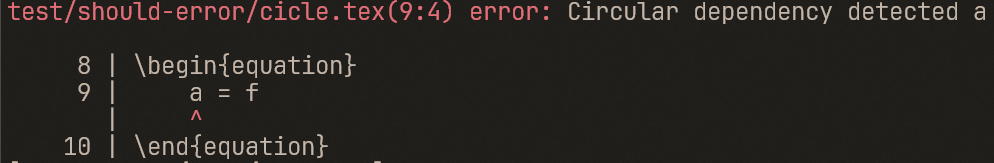
\includegraphics[scale=0.5]{./Imagens/error-circular-deps.png}
    \end{center}
\end{figure}


\subsection{Inferência de Tipos} \label{subsection-type-inference}


A função \verb`infer_type` determina o tipo de uma expressão (\verb`expr`) na AST durante a análise semântica, aplicando regras baseadas em operações matemáticas, como multiplicação entre número real e vetor, produto vetorial entre vetores e assinaturas de funções.

Projetada para processar todas as expressões de \texttt{EquationLang} — como identificadores, operadores, chamadas de função e literais —, a função verifica inicialmente se o tipo já foi inferido (\verb"expr.ty_inferred") para evitar processamento redundante. Caso contrário, realiza a inferência com base em um \verb"switch" que é capaz de avaliar todos tipos de expressões. Um trecho relevante desse processo está no \autoref{cod-type-inference}, que ilustra a discriminação e validação dos tipos.

Para \textbf{identificadores} (\verb"Expr_Identifier"), verifica-se se o identificador corresponde a um vetor especial, como $\omega_i$ ou $\vec{n}$. Nesse caso, o tipo é inferido como $\mathbb{R}^3$ (vetor tridimensional). Identificadores específicos, como \verb"\pi" ou \verb"\epsilon", são atribuídos ao tipo numérico real ($\mathbb{R}$). Para outros identificadores, a função consulta o escopo atual para determinar o tipo, com base nas estruturas detalhadas na \autoref{section-escope-table}.

\begin{codigo}[htb]
    \caption{\small Parte do switch da inferencia de tipos. }
    \label{cod-type-inference}
\begin{lstlisting}[language=C, frame=none, inputencoding=utf8]
infer_type :: proc(expr: ^ast.Expr, allow_invalid := false, default : ^ast.Type = ast.ty_invalid ) -> ^Type {
    /// Código omitido por brevidade  ///
    #partial switch e in expr.derived {
    case ^Expr_Identifier:
        // Alway set by the parser if indentifier starts with `\vec{}`
        if e.is_vector {
            type = new_type_vector(ty_number, 3) // vector 3 of type number (real)
        } else if e.identifier.kind == .Pi || e.identifier.kind == .Epsilon {
            type = ty_number
        } else {
            key := key_from_identifier(e)
            sym, ok := scope_get(key)
            if ok {
                if sym.type != nil {
                    type = sym.type
                }
            }
            /// Código omitido por brevidade  ///
        }

    case ^Expr_Prefix:
        right_type := infer_type(e.right, allow_invalid, default)
        /// Código omitido, mas aqui fazemos a validação da subexpressão direita e atribuimos o tipo correto para Expr_Prefix   ///

    case ^Expr_Infix:
        ty_left  := infer_type(e.left, allow_invalid, default)
        ty_right := infer_type(e.right, allow_invalid, default)
        /// Código omitido
        //  Inferimos tipo da expressão esquerda e direto dessa operação binária
        //  Depois validamos compatibilidade considerando a operação sendo usada nessas duas expressões

    /// Outros casos ...  ///
}
\end{lstlisting}
\end{codigo}


Para \textbf{operações prefixadas} (\verb"Expr_Prefix"), como raiz quadrada (\verb"\sqrt") ou funções trigonométricas (\verb"\sin", \verb"\cos"), a função valida se o operando é numérico e atribui o tipo correspondente à expressão. Nas \textbf{operações binárias} (\verb"Expr_Infix"), a função realiza a inferência dos tipos dos operandos esquerdo e direito. Se os tipos não forem compatíveis, aplica regras específicas. Alguma dessas regras são:

\begin{itemize}
    \item A multiplicação de um número por um vetor ($2*\vec{n}$) ou a divisão de um vetor por um número ($\frac{\vec{u}}{\sqrt{\vec{u} \cdot \vec{u}}}$) resultam no tipo vetor ($\mathbb{R}^3$).
    \item Operações entre dois números resultam em um número.
    \item Operações entre dois vetores resultam em um número ou um vetor a depender se a operação foi um produto vetorial ou produto interno.
\end{itemize}

Outros casos incluem \textbf{literais}, como números (\verb"Expr_Number") e vetores literais \\(\verb"Expr_Vector_Literal"), cujos tipos são atribuídos diretamente como $\mathbb{R}$ (números reais) e $\mathbb{R}^3$ (vetores tridimensionais), respectivamente.



Para chamadas de função (\verb"Expr_Function_Call"), o tipo da expressão é determinado pelo tipo do primeiro valor retornado pela função. A validação dos argumentos é realizada em outra função, detalhada na \autoref{subsubsection-eq-func-defn}. % ; Essa parte já foi dita
% Além disso, a função realiza validações específicas para evitar inconsistências, como garantir que operações entre vetores sejam semanticamente válidas (e.g., divisão entre vetores não é permitida).

% Em resumo, \verb`infer_type` é uma implementação robusta e flexível de inferência de tipos, essencial para a análise semântica de um compilador. A função assegura que cada expressão receba um tipo coerente com a semântica da linguagem, lidando com uma ampla gama de construções sintáticas e oferecendo suporte extensível para futuras adições à linguagem.

\subsection{Validação de Equações}

As declarações de equações são validadas após a coleta e ordenação descritas na \autoref{subsection-sym-resolution}, portanto assume-se que o lado esquerdo das equações seja um identificador válido ou uma definição de função e que estão na ordem correta de avaliação.

Qualquer violação semântica, como incompatibilidades de tipos ou uso de escalares onde vetores são esperados, é reportada ao usuário, com detalhes sobre o contexto e a localização do erro, conforme descrito em \autoref{subsection-erros}.

A função \verb"check_expr" realiza uma travessia semelhante à inferência de tipos e chama \texttt{infer\_type}. Nela, a análise de expressões que não foram feitas por \texttt{infer\_type} é realizada para todos os tipos de expressões. Algumas dessas validações estão listadas após este parágrafo, e um trecho dessa travessia pode ser visto no \autoref{eq-function-check-expr}.

\begin{itemize}
    \item \verb`Expr_Function_Call`: verifica se estamos fazendo a chamada corretamente com um identificador, evitando casos como tentar chamar uma função com um número, por exemplo, $123(x,y)$, o que é incorreto. Também checa se o número de argumentos corresponde ao número de parâmetros esperados.
    \item \verb`Expr_Prefix`: verifica operadores (\verb`-`, \verb`+`) e funções como \verb`sqrt(x)` e \verb`sin(x)`. Certifica-se de que os tipos sejam compatíveis, gerando erro em caso contrário, como quando um vetor é passado para a função seno.
    \item Literais de Vetor \verb`Expr_Vector_Literal`: garante que os vetores tenham exatamente 3 dimensões\footnote{Exigir vetores de apenas 3 dimensões pode ser considerado uma limitação semântica imposta pelo compilador}.
\end{itemize}




\begin{codigo}[H]
    \caption{\small Identificadores embutidos pela convenção deste trabalho.}
    \label{cod-builtins}
\begin{lstlisting}[language=C, numbers=none, frame=none, inputencoding=latin1]
BUILTIN_IDENTIFIERS :: []string {
    `\pi`,
    `\epsilon`,
    `\theta{h}`,
    `\vec{n}`,
    `\vec{h}`,
    `\vec{\omega{i}}`,
    `\theta{i}`,
    `\phi{i}`,
    `\vec{\omega{o}}`,
    `\theta{o}`,
    `\phi{o}`,
    `\theta{h}`,
    `\theta{d}`,
}
\end{lstlisting}
\end{codigo}


\begin{codigo}[H]
    \caption{\small Recorte da função \texttt{check\_expr}. }
    \label{eq-function-check-expr}
\begin{lstlisting}[language=C, basicstyle=\ttfamily\footnotesize, frame=none, inputencoding=utf8]
check_expr :: proc(expr: ^ast.Expr) {
    // Primeiro inferimos o tipo
    infer_type(expr)
    // Código omitido de preambulo
        case ^Expr_Identifier:
            // Check for using undefined indetifiers
            identifier_key := key_from_identifier(e)
            if !is_defined(e, false) {
                error(e.identifier,  "Identifier `%v` is not defined in the current scope.", identifier_key)
            }
        case ^Expr_Function_Call:
            check_expr(e.left)
            fn_ident, fn_ident_ok := e.left.expr_derived.(^ast.Expr_Identifier)
            if !fn_ident_ok {
                error(e.open,  "Tried to call an expression that is not an identifier")
            }
            fn_string := key_from_identifier(fn_ident)
            fn_sym, fn_sym_ok := scope_get(fn_string)
            fn_type, fn_type_ok := e.left.ty_inferred.derived.(^ast.Type_Function)
            if !fn_type_ok {
                error(e.open,  "Tried to call`%v`, which is not a function. Its type is `%v`", fn_string, format_type(e.left.ty_inferred))
            }
            if len(e.exprs) != len(fn_type.params) {
                error(
                    e.open,  "Args number mismatch. `%v` function expects  `%v` arguments but `%v` were given.",
                    fn_string, len(fn_type.params), len(e.exprs)
                )
            }
        // Outros casos omitidos
    }
}

\end{lstlisting}
\end{codigo}



\subsection{Validação de Funções}
A validação semântica de definições e chamadas de funções segue um processo semelhante ao da análise de expressões, mas com o uso da pilha de escopos.
Nas definições de funções, as variáveis no corpo da função são validadas para assegurar que todos os símbolos usados realmente estejam definidos no escopo da função. Já nas chamadas de funções, os argumentos fornecidos são comparados aos parâmetros esperados para validação.

\subsubsection{Definição de Funções} \label{subsubsection-eq-func-defn}

O procedimento \verb"check_function_definition" valida definições de funções, garantindo segurança de tipos e consistência através das seguintes tarefas:

\begin{enumerate}
    \item Inferir os tipos dos parâmetros.
    \item Inferir o tipo de retorno baseado na expressão final.
    \item Construir o tipo completo da função, incluindo parâmetros e retorno.
    \item Garantir que os identificadores usados estejam consistentes com seus tipos declarados.
    \item Validar as expressões no corpo da função.
    \item Criar um novo escopo para os parâmetros da função.
\end{enumerate}

O processo começa com o processamento dos parâmetros e o gerenciamento do escopo, como mostrado no \autoref{cod-parametros-validation}. Quando uma função é definida, um novo escopo é criado para armazenar informações dos parâmetros e da função, que são adicionadas ao escopo correspondente.

Esse escopo é essencial para validar chamadas de função e expressões no corpo. Cada função tem seu próprio escopo, com o escopo pai sendo o global, evitando conflitos de identificadores.

O controle de visibilidade funciona como esperado; se um parâmetro $x$ existe, ele é preferido ao $x$ global, resultando no fenômeno de \textit{shadowing}, como exemplificado na \autoref{eq-shadowing}, onde o valor de $f$ é 3, não 2.

\begin{align} \label{eq-shadowing}
    &x = 2 \\
    &g(x) = x \\
    &f = g(3)
\end{align}


Durante a validação dos parâmetros, cada identificador passa por um processo de inferência de tipo. Parâmetros marcados explicitamente com o prefixo \verb"\vec" recebem o tipo padrão $\mathbb{R}^3$ (vetor tridimensional), enquanto os demais são tratados como número real ($\mathbb{R}$).

Se um parâmetro $\vec{x}$ é declarado como vetor, todas as operações envolvendo $x$ no corpo da função devem respeitar as operações vetoriais; caso contrário, um erro será reportado.

\subsubsection{Chamada de Funções}
Chamadas de função passam por uma validação semelhante: os argumentos têm seus tipos inferidos e são comparados com a assinatura da função chamada (\verb"Type_Function").

No exemplo do \autoref{cod-type-mismatch}, a função $g$ possui a assinatura $\mathbb{R} \times \mathbb{R} \to \mathbb{R}$. A expressão resultante da chamada de função terá o tipo do contradomínio da função. Também é necessário confirmar que $g$ refere-se a um símbolo do tipo função.

\begin{codigo}[H]
    \caption{\small Equação com uso incorreto de tipos na chamada de função.}
    \label{cod-type-mismatch}
\begin{lstlisting}[language=tex, numbers=none, frame=none, inputencoding=latin1]
\begin{equation}
    g(a, x) = a*x*x
\end{equation}

\begin{equation}
    f = g(1, \vec{1,1,1})
\end{equation}

\end{lstlisting}
\end{codigo}

A função $g$ espera dois números reais como argumentos, mas na equação $f$, um vetor foi passado no lugar de um número, o que gera um erro. A \autoref{fig-type-mismatch} ilustra esse erro, indicando a função com o argumento incompatível. Além disso, ao passar os argumentos, também validamos se a quantidade de argumentos corresponde ao número de parâmetros esperados.

\begin{figure}[H]
    \caption{\label{fig-type-mismatch} \small Erro gerado por uso incorreto de tipos na chamada de função.}
    \begin{center}
        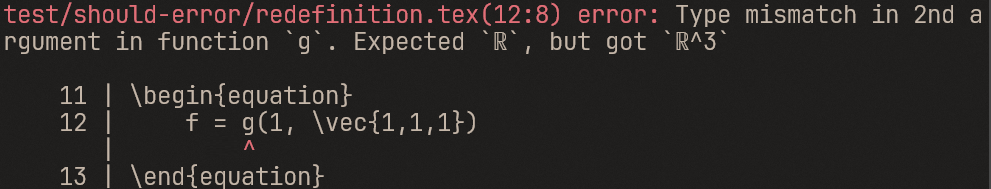
\includegraphics[scale=0.5]{./Imagens/error-type-mismatch.png}
    \end{center}
\end{figure}


\begin{codigo}[H]
    \caption{\small Validação de parâmetros de uma função.}
    \label{cod-parametros-validation}
\begin{lstlisting}[language=C, numbers=none, frame=none, inputencoding=latin1]
// ...
parameter_types := [dynamic]^Type{}
scope_enter(fn_sym.scope) {
    for &parameter in fn.parameters {
        parameter_key := key_from_identifier(parameter)
        ty := infer_type(parameter, true, ty_number)
        parameter_sym.type = ty
        append(&parameter_types, ty)
    }
}
// ...
\end{lstlisting}
\end{codigo}

%
% \begin{codigo}[htb]
%     \caption{\small Gerenciamento de escopo na validação do corpo da função.}
%     \label{cod-scope-management}
% \begin{lstlisting}[language=C, numbers=none, frame=none, inputencoding=latin1]
% scope_enter(fn_sym.scope) {
%     // Validação do corpo da função
%     check_expr(body)
%     // Inferência e validação de tipo
%     body_type := infer_type(body)
% }
% \end{lstlisting}
% \end{codigo}

%
% \begin{codigo}[htb]
%     \caption{\small .}
%     \label{cod-types-structs}
% \begin{lstlisting}[language=C, numbers=none, frame=none, inputencoding=utf8]
% case ^Decl_Equation:
%     check_decl(s)
%
% scope_enter(fn_sym.scope) {
%     // Validação do corpo da função
%     check_expr(body)
%     // Inferência e validação de tipo
%     body_type := infer_type(body)
%     result_types := [dynamic]^Type{body_type}
%     fn_type := make_function_type(parameter_types[:], result_types[:])
% }
% \end{lstlisting}
% \end{codigo}

